\documentclass[a4paper,12pt]{article}
\usepackage{tikz}
\usetikzlibrary{mindmap,trees}
\begin{document}

\title{CSP:301  Monopoly with a twist}
\author{Robin Malhotra}
\date{August 12, 2014}
\maketitle

\section{Introduction}
This is the design document for the CSP301 course at IIT Delhi(Fall Semester,2014).
In this course, our main aim is to create a video game version of the popular board game Monopoly. The game has to run independently on OSX, Windows and Linux with no modifications.

\section{Parts of the project}
Instead of a huge list, I find it easier to use a visual mindmap of the course.

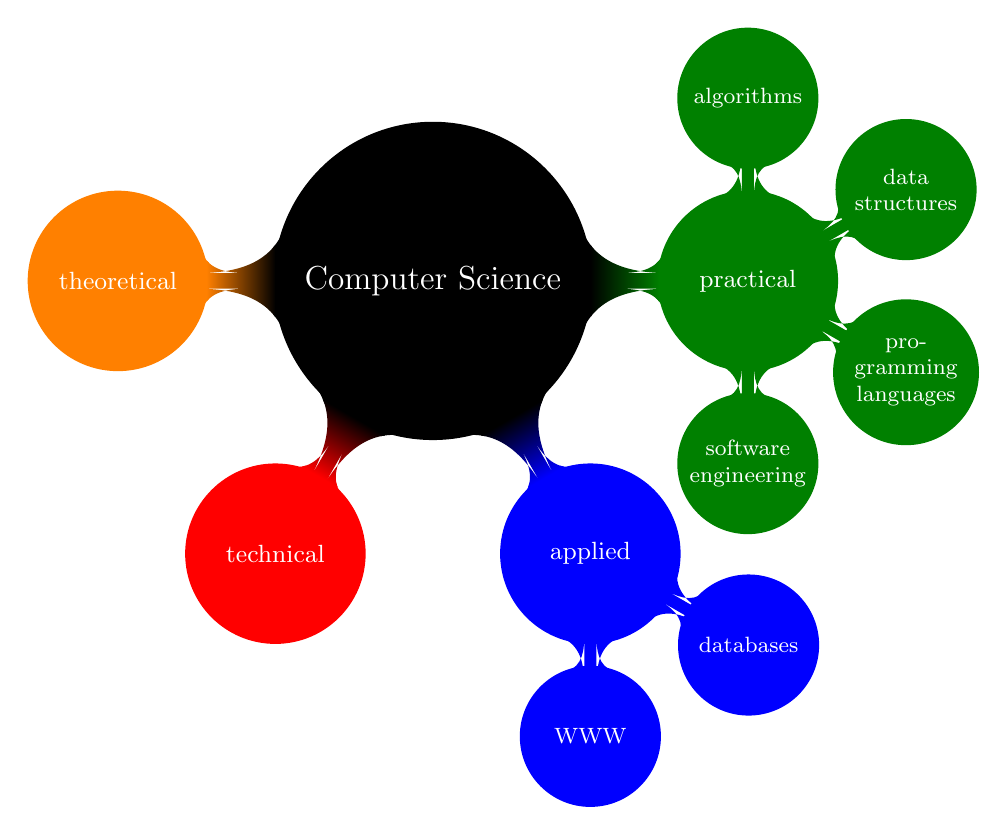
\begin{tikzpicture}[scale=0.8]
  \path[mindmap,concept color=black,text=white]
    node[concept] {Computer Science}
    [clockwise from=0]
    child[concept color=green!50!black] {
      node[concept] {practical}
      [clockwise from=90]
      child { node[concept] {algorithms} }
      child { node[concept] {data structures} }
      child { node[concept] {pro\-gramming languages} }
      child { node[concept] {software engineer\-ing} }
    }  
    child[concept color=blue] {
      node[concept] {applied}
      [clockwise from=-30]
      child { node[concept] {databases} }
      child { node[concept] {WWW} }
    }
    child[concept color=red] { node[concept] {technical} }
    child[concept color=orange] { node[concept] {theoretical} };
\end{tikzpicture}

\end{document}